%\RequirePackage[l2tabu, orthodox]{nag}
\documentclass[a4paper,12pt]{scrreprt}
\usepackage[utf8]{inputenc}
\usepackage[T1]{fontenc}
\usepackage[english]{babel}		% English language 
%\usepackage[backend=bibtex,style=authoryear,bibstyle=nature,natbib=true]{biblatex}
%--------------------------------------------------
% if using biblatex
%\usepackage{csquotes}
%--------------------------------------------------
\usepackage{color}						% enable color
\usepackage{graphicx}					% fancy graphics
\usepackage{lmodern}					% font looks better on screen
\usepackage{microtype}				% improve kerning
\usepackage{natbib}           % bibliography for scientists
%--------------------------------------------------
% more features
%\usepackage{enumerate}				% customize numbered lists
\usepackage{amsmath}					% all the fancy math stuff
\usepackage{listings}         % code listings
%\usepackage{tabularx}         % extended tables
%\usepackage{tikz}             % draw stuff with tikz
\usepackage{url}							% URL handling
\usepackage{xspace}						% to space or not to space
\usepackage{hyperref} 				% should be loaded last
%--------------------------------------------------

% setup biblatex
%--------------------------------------------------
% \bibliography{bib/diploma}
% \ExecuteBibliographyOptions{
% 	firstinits=true,
% 	backref=true,
% 	isbn=false,
% 	url=false,
% 	maxcitenames=2,
% 	maxbibnames=999,
% }
%-------------------------------------------------- 

% setup natbib citation format
\bibpunct{(}{)}{,}{a}{,}{,}

% setup the listings package
\lstset{%
	language=perl,
	basicstyle=,                       % the size of the fonts that are used for the code
	numbers=left,                      % where to put the line-numbers
	numberstyle=\tiny,                 % the size of the fonts that are used for the line-numbers
	%stepnumber=2,                      % the step between two line-numbers. If it is 1 each line will be numbered
	numbersep=5pt,                     % how far the line numbers are from the code
	backgroundcolor=\color{lightgrey}, % choose the background color. You must add \usepackage{color}
	showspaces=false,                  % show spaces adding particular underscores
	showstringspaces=false,            % underline spaces within strings
	showtabs=false,                    % show tabs 
	frame=none,                        % can be: none, leftline, topline, bottomline, lines, single, shadowbox 
	%frameround=tttt,                   % rounded corners; t=round, f=corner
	tabsize=2,                         % sets default tabsize to 2 spaces
	captionpos=t,                      % caption position (t|b)
	breaklines=true,                   % automatic line breaking
	breakatwhitespace=false,           % automatic breaks should not happen at whitespace
	%escapeinside={\%}{)}               % if you want to add a comment within your code
}

% setup hyperlinks, bookmarks and pdf metadata
\hypersetup{%
	bookmarks=true,
	pdfborder={0 0 0},
	pdftitle={Fast and efficient mapping of transcript sequences to ortholog groups},
	pdfauthor={Malte Petersen},
	pdfcreator={pdflatex},
	pdfsubject={orthology prediction},
	pdfkeywords={orthology} {prediction} {est} {transcriptome} {hmm} {phylogenetics} {thesis} {1kite}
}
% alleviate compression so pdftk won't complain
\pdfobjcompresslevel=1

% new colors and commands
\definecolor{lightgrey}{rgb}{0.9,0.9,0.9}
\newcommand{\file}[1]{{\lstinline{#1}}}
\newcommand{\code}[1]{{\texttt{#1}}}
\newcommand{\hamstr}{HaMStR\xspace}
\newcommand{\pname}{Orthograph\xspace}
\newcommand{\species}[1]{\textit{#1}}
\newcommand{\todo}[1]{\textbf{\color{red}[#1]}}

% doublespace
\linespread{1.3}

\title{Fast and efficient mapping of transcript sequences to ortholog groups}
\author{Malte Petersen}

\begin{document}
\maketitle
\pagestyle{headings}
\tableofcontents

\chapter*{Paper notes}
	\todo{where do I put hmmtest?}

Strategies for orthology prediction:

Tree reconciliation

\begin{itemize}
	\item topology of a gene tree compared with that of the chosen species tree
	\item reconciled by maximum parsimony $\rightarrow$ reflects ortholog
		relationships
	\item genome-wide application precluded by:
	\begin{itemize}
		\item horizontal gene transfer, especially in prokaryotes (widespread HGT
			invalidates the very notion of a species tree)
		\item computationally expensive
	\end{itemize}
\end{itemize}

\begin{description}
	\item[\cite{mirkin1995}] Tree-based approach to orthology prediction
	\item[\cite{page1998}] Tree reconciliation method
	\item[\cite{yuan1998}] Tree-based approach to orthology prediction
	\item[\cite{kuzniar2008}] Review of approaches
\end{description}

most studies employ simplifications/shortcuts $\rightarrow$ graph-based approaches:

Triangulation

\begin{itemize}
	\item OrthoDB 
	\item COG (KOG, EGO, etc)
\end{itemize}

Reciprocal best hit (RBH) 

\begin{itemize}
	\item RBH strategies recover only one-to-one orthologs (the bidirectional best
		hit)
	\item InParanoid (BLAST based)
\end{itemize}

Markov clustering:

\begin{itemize}
	\item OrthoMCL
\end{itemize}

Homoplasy: similarity in unrelated organisms. Homoplasies demonstrate adaptation
in the living world.

Homoplasy \citep{lankester1870}: It may be said that the term ``analogy'',
already in use, is sufficient to indicate what is here termed ``homoplasy''; but
analogy has had a wider signification given to it, in which it is found very
useful to employ it, and if could not be used with any accuracy in place of
homoplasy.  \emph{Any} two organs having the same function are analogous,
whether closely resembling each other in their structure and relation to other
parts or not, and it is well to retain the word in that wide sense. Homoplasy
includes all cases of close resemblance of form which are not traceable to
homogeny, all \emph{details} of agreement not homogenous, in structures which
are broadly homogenous, as well as in structures having no genetic affinity.


\thispagestyle{empty}
\null
\vfill
\begin{quote}
	\emph{Mutation:} it is the key to our evolution. It has enabled us to evolve
	from a single-celled organism into the dominant species on the planet. This
	process is slow, and normally taking thousands and thousands of years. But
	every few hundred millennia, evolution leaps forward.\\
	\null\hfill--- \citet{singer2000}
\end{quote}


\chapter{Introduction}
	Since the advent of DNA sequencing technology and the reconstruction of
genealogical relationships based on nucleic or amino acid sequences, the
challenge has arisen to select appropriate, comparable molecular characters for
phylogenetic analyses. So-called orthologs are the only type of molecular
characters that can be used as evidence of a speciation event. 

A number of techniques has been developed to assess orthology in genomes. In
recent research, transcriptomes---which are only the subset of a genome that is
expressed at the time of RNA preservation---are frequently used because of lower
sequencing cost. However, methods that work in whole genomes cannot be applied
to transcriptomes because of the inherent incompleteness of transcriptomic data.
In the present thesis, I outline the concept of gene orthology and infer a
software pipeline that allows orthology prediction in transcriptome data.


	\section{Orthology}
		When reconstructing the evolution of species lineages, so called homologous
characters are used to reconstruct phylogenetic trees. The term homolog was
introduced by \citet{owen1848} and was used to describe ``the same organ in
different animals under different every variety of form and function''.
Similarly, analogs were defined as ``part or organ in one animal which has the
same function as another part or organ in a different animal''. At that time,
Owen had no notion of the concept of evolution, and in the famous \emph{Origin
of Species} \citep{darwin1859}, the term homology is never used. However, in a
review, \citet{owen1860} refers to homology as evidence of evolution.

A morphological character is the phenotypic reflection of genetic information.
Since the analysis of molecular data entered the field of phylogenetics during
the 1960s, these are used in numerous studies on species relationships.
Molecular characters, such as the DNA sequences of genes, are homologous if they
share a common origin. However, this is not sufficient to infer reliable
phylogenies based on molecular sequence data. Genes do not only dplicate during
a speciation event, but can be subject to a number of events in the course of
their evolutionary history, such as speciation, gene duplication, gene loss,
horizontal gene transfer as well as fusion, fission and other rearrangements of
genes \citep{koonin2005}.  These different types of relatedness between
sequences of molecular characters have made new definitions necessary (see
\autoref{fig:orthology}).

\begin{figure}[h]
	\centering
	\def\svgwidth{0.8\textwidth}
	\input{img/orthology-paralogy.pdf_tex}
	\caption[Orthology, paralogy, and xenology]{Subtypes of homology. The red
		arrow denotes horizontal gene transfer; AB1 is \emph{xenologous} to all
		other genes. B1 and C1 are \emph{orthologs}. Both C2 and C3 are
		\emph{inparalogs} to each other but \emph{co-orthologs} to B2, as are B1 and
		C1 compared to A1. B1 and B2 are outparalogs. Graphic adapted from
		\citet{fitch2000}.
	}
	\label{fig:orthology}
\end{figure}


Homologous genes in two or more species that are related by a speciation event
are called \emph{orthologs}\footnote{\emph{ortholog} n., \emph{orthologous}
adj.; the other terms are flexed accordingly.} \citep{fitch1970}. They reflect
species phylogeny directly and are most commonly used to infer phylogenetic
relationships between species. \emph{Paralogs} are also homologous genes, but
they are related by a gene duplication event within a species and are not
involved in horizontal radiation \citep{ohno1970}. Further distinction must be
made among paralogous genes \citep{remm2001}: paralogous genes that are related
by a lineage-specific duplication are called \emph{outparalogs} if the
duplication occurred prior to a given speciation event. On the contrary, genes
that result from a lineage-specific duplication subsequent to a given speciation
event are called \emph{inparalogs}. Additionally, two genes in a single species
that are paralogous to each other can be \emph{co-orthologs} to a gene in
another species. These distinctions are important when looking at internal
branches of a phylogenetic tree. 

A fourth subtype of homology is called \emph{xenology}. It is defined as the
condition in which the history of the genes involves horizontal, or
interspecies, gene transfer \citep{gray1983}. This is the only form of homology
in which the gene lineage cannot be traced back to a parent, but instead from
one organism to another.

In molecular phylogenetics, orthologous molecular sequences are used to
reconstruct genealogical relationships, because these sequences are the only
homologous sequences whose phylogeny reflects the genealogical relationships of
the species from which the sequences were obtained. Orthologs are also used to
study mechanisms of gene and genome evolution \citep{dessimoz2012}. Orthologs
tend to be more functionally similar than paralogs \citep{altenhoff2012}. This
is the so-called \emph{ortholog conjecture} \citep{tatusov1997}, and the reason
why the analysis of protein families often relies on orthology among the
investigated genes. In addition, housekeeping genes, i.e., genes that are
essential to keeping an organism alive, underlie stronger sequence conservation
due to selection pressure \citep{she2009} and are more likely to be orthologous
across species \citep{waterhouse2011}. 

	\section{How can orthology be assessed?}
		With next-generation, high-throughput technologies providing vast amounts of
sequence data, 

To make use of the information contained in the ortholog property, it is
important to classify conserved genes according to their homologous
relationships. It is worth mentioning here that homology is a concept of
quality, not quantity (\cite{reeck1987}) and thus indivisible. Two sequences can
be \emph{similar} by a percentage (e.g., amino acid positional identity), but
they are either homologous or they are not. The same follows for orthologs,
paralogs, and xenologs. This distinction is important because homology implies a
genealogical relationship, whereas similarity does not. Similarity can also be
the result of other evolutionary processes, such as convergence, which results
in \emph{analogy}. All variants of similarity can be grouped under the term
\emph{homoplasy}, which encompasses similarity (\emph{homos} (``equal''),
\emph{plasis} (``shaping'')) excluding homology and its subforms. In the present
thesis, the definition of homoplasy is used as it appears in \cite{page1998}.

A simple alignment or scoring (i.e., similarity) alone cannot separate
homologous from merely similar sequences (\cite{eisen1998}). To distinguish
homology from homoplasy, further logic is necessary: 

See figure \ref{fig:hamstr}.

	\section{Transcriptomes and additional challenges}
		Going a step back and asking why genomes are studied, many times the answer is
that one wants to understand the function of genes and proteins. The genome is
made up of long strands of deoxyribonucleic acid (DNA). It contains the
necessary instructions to create and maintain cells.  Proteins are produced
according to information on the DNA in a two-step process: during
\emph{transcription}, messenger ribonucleic acid (mRNA) is synthetisized. In the second step, \emph{translation}, the
mRNA is used by specialized organelles, namely ribosomes, to synthetisize
proteins from amino acids. In eukaryotes, this process includes \emph{splicing},
during which non-coding regions, so-called \emph{introns} are removed from the
mRNA. In bacteria and archaea, the mRNA requires typically no further processing
before translation. The resulting molecule contains only \emph{exons}, coding
regions of the genome that are relevant for translation. The ratio of exons to
introns varies across organisms; \eg, the human genome consists of only 1.1\% to
1.4\% exons and 24.4\% to 37.8\% introns, the rest is intergenic DNA
\citep{venter2001}. That means that in eukaryotes, the majority of the genome
does not code for proteins, and the functional analysis of the genes in an
eukaryote genome requires screening the nucleotide sequence data for those
non-coding regions.

The study of \emph{transcriptomes} circumvents these problems. A transcriptome
is the collection of all transcripts in a tissue sample at the time of RNA
preservation.  Transcriptomes are frequently used in phylogenetics and
phylogenomics to reconstruct species trees based on hundreds of
genes\footnote{The 1KITE project (1K Insect Transcriptome Evolution,
\url{http://1kite.org}) aims to sequence the transcriptomes of 1,000 insect
species and infer a robust backbone tree of insects. Preliminary analyses were
performed on a supermatrix of 1,478 genes.}.  The combination of low-cost
next-generation sequencing and the intron-free nature of transcriptomes allow
access to a high proportion of protein coding genes per sequenced mega-base pair
at a fraction of the cost for sequencing the corresponding genome.

Next-generation transcriptome sequencing technologies achieve their high
throughput by massively parallelizing the sequencing process. They cannot
sequence whole genomes in a single run, but produce a large number of so-called
\emph{reads}, short nucleotide sequences (20 to 1,000 bp in length, depending on
the technology used).  These fragments must be \emph{assembled} to form
so-called \emph{contigs}, contiguous sequences of nucleotides that most closely
resembles the nucleotide sequence present in the sequenced specimen. The
assembly process is a computationally complex problem that has not yet been
solved to perfection.  Reviews of different strategies have been written by,
\eg, \citet{zhang2011}.  The assembled data may be redundant due to, \eg,
alternative splicing products \citep{black2003} or multiple, non-overlapping
sequencing of C-terminus and N-terminus (the two ends of a DNA strand or gene).
Most assembly software cannot detect these issues reliably \citep{haiminen2011}. 

In addition to the processes explained above, next-generation transcriptome
sequencing and assembly output sequence data are not only fragmented and
possibly redundant (overlapping), but most importantly they are
\emph{incomplete} because not all genes may have been expressed at the time of
preservation. Due to this inherent incompleteness of transcriptomes, orthology
prediction approaches that are used on fully sequenced and annotated genomes
cannot be used.

\begin{figure}[t]
	\centering
	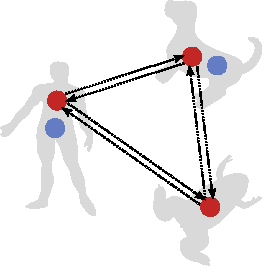
\includegraphics[width=0.4\textwidth]{img/triangulation-bbh.pdf}
	\caption[Bidirectional best hit (BBH) triangulation]{
		Bidirectional best hit (BBH) triangulation. To identify genes as orthologous
		in the presence of potential gene loss or incomplete data, they must be BBH
		in three species.  In this example, the red gene fulfills this criterion.
		The blue gene cannot be unambiguously identified as orthologous, as it is
		not present in the frog and paralogy is possible (compare to
		\autoref{fig:graph-based-strat}).  Graphic modified from
		\citet{altenhoff2012}.
	}
	\label{fig:triangulation-bbh}
\end{figure}


When performing a bidirectional search on a fully sequenced and annotated
complete genome as described above, it can happen that two genes that are
identified as BBH are paralogs because the corresponding orthologs have been
lost in both investigated species. This situation is called \emph{differential
gene loss}\cite{altenhoff2012} and best solved using a tree-based approach. In
the face of the aforementioned difficulties of a tree-based strategy, some
graph-based algorithms implement \emph{triangulation}
(\autoref{fig:triangulation-bbh}): to identify two genes as orthologous, they
must be BBH not only in two, but in three species. The third gene functions as
possible ``witness of non-orthology'' \citep{dessimoz2006}. A triangulation
strategy can also be applied to orthology prediction in transcriptomic data, the
incompleteness of which may be seen as a similar situation as potential gene
loss in fully sequenced and annotated genomes. This approach has been
implemented in \hamstr \citep{ebersberger2009}, which I will describe in the
following section.

	\section{\hamstr}
		HaMStR \citep{ebersberger2009} implements a graph-based approach using hidden
Markov models (HMMs, see section \ref{sec:hmms}). It is aimed specifically at
searching for orthologs in expressed sequence tag (EST) data, which is sequenced
using complementary DNA (cDNA) libraries. This cDNA is generated from mRNA and
therefore contains no introns. EST data can be redundant and fragmented, which
is why methods for orthology prediction in genomic data cannot be applied.

The HaMStR algorithm goes as follows:

\begin{enumerate}
	\item For each HMM, do the following:
		\begin{enumerate}
			\item Search the EST library. If matches were found, do the following for
				each:
			\begin{enumerate}
				\item Search the hit sequence against a BLAST database of all reference
					proteomes (the ``reciprocal BLAST''). 
				\item If matches were found: 

			\end{enumerate}
		\end{enumerate}
\end{enumerate}

\begin{figure}[h]
	\centering
	\def\svgwidth{0.8\textwidth}
	\input{img/triangulation.pdf_tex}
	\caption[Triangulation]{Triangulation:
		\begin{inparaenum}
			\item The transcript sequence space is searched using a hidden Markov
				model (HMM), which is a statistical representation of the reference
				sequences that were used to build it.
			\item A reference proteome is searched using the match sequence from the
				HMM search (reciprocal search).
			\item If the reciprocal search match sequence is one that was used to
				build the HMM, then orthology is assumed.
		\end{inparaenum}
	}
	\label{fig:hamstr}
\end{figure}

% enable this if you need it, it makes compilation a bit slower
%\usetikzlibrary{shapes,arrows}
\tikzstyle{rect} = [
	rectangle,
	draw,
	fill = green!15,
	text width = 9 em,
	text centered,
	minimum height = 3 em,
]
\tikzstyle{block} = [
	rectangle,
	draw,
	fill = blue!20,
	text width = 13em,
	text centered,
	rounded corners,
	minimum height = 3em,
]
\tikzstyle{decision} = [
	diamond,
	draw, 
	fill = blue!20, 
	text width = 4.5em,
	text centered,
	node distance = 14em,
	inner sep = 0pt
]
\tikzstyle{line} = [draw, -latex]
\tikzstyle{cloud} = [
	draw,
	ellipse,
	fill = red!20,
	text width = 7.5em,
	text badly centered,
	node distance = 3cm,
	minimum height = 2em
]

\hyphenation{ref-e-ren-ce tran-scrip-to-me or-tho-lo-gous}
\begin{tikzpicture}[node distance = 2cm, auto]
	% nodes
	\node[rect] (transcriptome) {Transcriptome library};
	\node[block, below of = transcriptome] (hmmsearch) {Search transcriptome library using next HMM};
	\node[rect, left of = hmmsearch, node distance = 14em] (orthologs) {pHMMs of orthologous sequences};
	\node[block, above of = orthologs] (orthodb) {Orthologous sequences of reference taxa from OrthoDB};
	\node[block, below of = hmmsearch, node distance = 4em] (hmmhits) {BLAST result(s) against next reference taxon};
	\node[decision, below of = hmmhits, node distance = 7em] (blast) {BLAST hit in HMM?};
	\node[rect, right of = hmmhits, node distance = 14em] (proteomes) {Proteomes of the reference taxa};
	\node[cloud, below of = blast, node distance=7em] (orthologous) {Orthologous, save \& process};
	\node[decision, below of = orthologous, node distance = 6em] (hmmsleft) {HMMs left?};
	\node[decision, left of = blast, node distance = 16em] (reftaxaleft) {Reference taxa left?};
	\node[cloud, below of = reftaxaleft, node distance = 7em] (notorthologous) {Not orthologous, discard};
	\node[draw, below of = hmmsleft, node distance = 6em] (end) {End};

	% lines
	\path[line](transcriptome) -- (hmmsearch);
	\path[line](orthodb) -- (orthologs);
	\path[line](orthologs) -- (hmmsearch);
	\path[line](hmmsearch) -- (hmmhits);
	\path[line](proteomes) -- (hmmhits);
	\path[line](hmmhits) -- (blast);
	\path[line](blast) -- node[near start]{no} (reftaxaleft);
	\path[line](blast) -- node[near start]{yes} (orthologous);
	\path[line](orthologous) -- (hmmsleft);
	\path[line](hmmsleft) -| node[near start]{yes} ([xshift = 18.0em]hmmsleft.east) |- (hmmsearch);
	\path[line](reftaxaleft) |- node[near start]{yes} (hmmhits);
	\path[line](reftaxaleft) -- node[near start]{no} (notorthologous);
	\path[line](notorthologous) |- (hmmsleft);
	\path[line](hmmsleft) -- node[near start] {no} (end);
\end{tikzpicture}


		\subsection{Hidden Markov models}
			\label{sec:hmms}
Biological molecular sequences such as amino acid and nucleotide sequences can
usually be classified into families that share homologous features, \eg, a
similar three-dimensional structure or a particular sequence of amino acids
\citep{henikoff1997}. Since a similarity measure bears no genealogical
meaning---as explained in \autoref{sec:orthology-howto}---more appropriate
approaches must be employed to identify homology.

Hidden Markov models (HMMs) are statistical models that are particularly well
suited to process so-called ``linear'' problems. Because of this property, HMMs
have seen widespread use in temporal pattern recognition algorithms, such as
speech and gesture recognition or musical score following for over thirty years
\citep{rabiner1989}. They were introduced into computational biology by
\citet{churchill1989} and used as profile models since the 1990s
\citep{krogh1994}. Their statistical, linear nature makes them very useful for
application on nucleic or amino acid sequences, which are usually linear and can
be modelled in such a fashion. 

The basis of a HMM is a stochastic process called Markov chain, which was named
after the mathematician Andrey Markov who described them in the late 19th
century. A Markov chain is a sequence of states $s_{i1}, s_{i2}, ...  s_{ik},
...$ that is generated by a process that transits with a certain probability
from one state to the next. The probability of each subsequent state depends
only on the previous state:

\begin{equation}
P(s_{ik} | s_{i1}, s_{i2}, ..., s_{ik-1}) = P(s_{ik} | s_{ik-1})
\label{eqn:markov-chain}
\end{equation}

For example, in a simple Markov chain with the two possible states ``rain''
($s_1$) and ``dry'' ($s_2$) that have the transition probabilities $P(s_1|s_1) =
0.3$, $P(s_2|s_2) = 0.2$, $P(s_2|s_1) = 0.7$, $P(s_1|s_2) = 0.8$, and the
initial probabilities $P(s_1) = 0.4$, $P(s_2) = 0.6$, the probability of the
state sequence ``dry'', ``dry'', ``rain'', ``rain'' is

\begin{equation}
	\begin{split}
		P(\{s_2, s_2, s_1, s_1\}) &= P(s_2) P(s_2|s_2) P(s_1|s_2) P(s_1|s_1) \\
		&= 0.6 \cdot 0.8 \cdot 0.2 \cdot 0.3 
	\end{split}
\label{eqn:markov-chain-weather}
\end{equation}

or, written more generally

\begin{equation}
	\begin{split}
		P(s) &= P(s_L|s_{L-1}) P(s_{L-1}|s_{L-2}) . . . P(s_2) P(s_1) \\
		&= P(s_1) \prod^{L}_{i=2}a_{s_{i-1}s_{i}}
	\end{split}
	\label{eqn:markov-chain-general}
\end{equation}

where $a$ is the transition probability from one given state to the next and $L$
is the length of the sequence.

In a \emph{hidden Markov model} (see \autoref{fig:hmm} on page \pageref{fig:hmm}), there are multiple chains that are invisible to
the observer, and only its output can be interpreted. A simple HMM consists of a
two-state Markov chain that \emph{emits} a sequence of characters, \eg, nucleotide
symbols, each with a probability that is dependent on the state of the chain. The state chain
transits between two states that have different emission probabilities for the
four possible symbols. Only the output sequence is visible to the observer, the
state sequence remains hidden.
% However, using stochastic theory, it can be inferred.
Generally, a HMM generates a state sequence as follows: First a state $s_1$ is
chosen according to the probabilities $a_{0i}$. Then a new state $s_2$ is
chosen according to the transition probabilities $a_{s_{1}i}$ and so forth
\citep{durbin1998}. The general joint probability of an observed sequence $x$
and a state sequence $s$ is written as follows:

\begin{equation}
P(x,s) = a_{0s_1} \prod_{i=1}^L e_{s_i}(x_i)a_{s_is_{i+1}}
\label{eqn:hmm-general}
\end{equation}

where $a_{s_{L+1}} = 0$ is required. Equation \eqref{eqn:hmm-general} is the HMM
analogue of equation \eqref{eqn:markov-chain-general} \citep{durbin1998}.

\begin{figure}[h!]
	\centering
	\def\svgwidth{\textwidth}
	\input{img/hmm-eddy.pdf_tex}
	\caption[A simple hidden Markov model]{A simple, two-state hidden Markov model
		(HMM) describing a DNA sequence with a heterogeneous base composition. 
		\textbf{a)} State 1 generates AT-rich sequences. State 2 generates CG-rich
			sequences (so-called CpG islands). State transitions and their respective
			probabilities are indicated by arrows. Symbol emission probabilities for
			each state are listed below the states. State transition probabilities
			and emission probabilities are model parameters.
		\textbf{b)} At each position, the model not only emits a symbol (\eg, a
			nucleotide character) with a probability that is dependent on its state, it
			also transits to the other state with a certain probability, or remains in
			the present state.
		\textbf{c)} The symbol sequence is the result of the state transitions and
			the emission probabilities in those states. 
		Graphic from \citet{eddy1996}.
	}
	\label{fig:hmm}
\end{figure}



\clearpage

HMMs can be used in a pairwise sequence alignment algorithm using transition
scores: the transitions are assigned a score increment according to the
transition probabilities, and the resulting states each specify a $\Delta(i,j)$
pair for the transition from $s_i$ to $s_j$. The alignment algorithm uses a
\emph{finite state automaton} (FSA), which is a concept from computer science
and describes an abstract machine that can be in one of a finite number of
states. A FSA is defined by a list of its states and the triggering condition
for each transition, and can be described with a HMM. An alignment corresponds
to a path through the states, with symbols from the underlying pair of
sequences (which can also be gaps) being transferred to the alignment according
to the $\Delta(i,j)$ values in the states \citep{durbin1998}. 

\todo{elaborate}

HMM-based alignment algorithms have been demonstrated to be very effective in
detecting conserved patterns in multiple amino acid sequences \citep{eddy1995,
hughey1996}.  This performance is achieved by \emph{training} the HMM on a
multiple sequence alignment of amino acid sequences (when attempting to align
amino acid sequences) that are members of a protein family. The resulting HMM
can discriminate between protein family members and non-family members with
great accuracy, even if they are very remotely related to each other
\citep{karplus1998}. In the HMMER3 implementation (see \autoref{sec:programs}),
HMM searches exhibit a better specificity---that is, a better ratio of
$\textrm{[true positives/true positives+false negatives]}$
\citep{korf2004}---than both BLAST \citep{altschul1990} and PSI-BLAST
\citep{altschul1997} (benchmark tests by \citet{eddy2009}).


		\subsection{Room for improvements}

\chapter{Material and methods}
	\section{Hardware}
		All analysis steps were performed on a standard desktop computer equipped with
an Intel \mbox{Core 2 Duo} E8500 clocked at 3.16 GHz and 4 GB of RAM
running Fedora Linux with the most recent 64-bit kernel (3.6.10 at the time of
this writing). 

	\section{Programs}
		\label{sec:programs}
The programs listed in table \ref{tab:programs} were used in this project and
are described in the following subsections. For all compilation steps, the GNU C
compiler (\nomenclature{GCC}{Gnu C compiler}) was used.

\begin{table}
	\caption[Programs used in this project]{Programs used in this project. Versions may not be the latest at the time of writing, as development and improvement on them is still ongoing.}
	\begin{tabularx}{\textwidth}{p{0.13\textwidth} p{0.1\textwidth} p{0.6\textwidth}}
	\hline
	Package   & version & downloaded from \\
	\hline
	BLAST+    & 2.2.25+ & \url{ftp://ftp.ncbi.nlm.nih.gov/blast/executables/blast+/LATEST/} \\
	Exonerate & 2.2.0   & \url{http://www.ebi.ac.uk/~guy/exonerate/} \\
	GCC       & 4.7.2   & \url{http://gcc.gnu.org} \\
	HMMER3    & 3.0     & \url{http://hmmer.janelia.org} \\
	MySQL     & 5.5.28  & \url{http://mysql.com} \\
	Perl      & 5.14.3  & \url{http://www.perl.org} \\
	\end{tabularx}
	\label{tab:programs}
\end{table}



		\subsection{HMMER3}
			HMMER3 (\cite{eddy2011}) is written in C and published under the GNU General
Public License (GPL). It is available in binary form for 32-bit and 64-bit
platforms and as source code from the site of the developers.  I downloaded the
source code, compiled it with the GNU C compiler (GCC) and installed the binaries
locally. 

		\subsection{BLAST+}
			The Basic Local Alignment Search Tool BLAST \citep{altschul1990} searches for
regions of local similarity between nucleotide or amino acid sequences. The
program compares nucleotide or amino acid sequences to databases of amino acid
or nucleotide sequences and calculates the statistical significance of matches.
BLAST can be used to infer functional and evolutionary relationships between
sequences as well as help identify members of gene families (description from
\url{http://blast.ncbi.nlm.nih.gov}).

The NCBI BLAST+ package is written in C++ and published under a public domain
license. It is available in binary form for various 32-bit and 64-bit platforms
as well as in source code from the NCBI website. I downloaded the 64-bit Linux
binary version and installed it locally.

		\subsection{Exonerate}
			Exonerate \citep{slater2005} is a generic tool for pairwise sequence comparison.
It allows sequence alignments using many alignment models, using either
exhaustive dynamic programming, or a variety of heuristics (description from
\url{http://www.ebi.ac.uk/~guy/exonerate}). In contrast to its predecessor
Genewise \citep{birney2004}, which is no longer under development, Exonerate is
not only faster by a two-digit factor depending on the data, but also allows
frameshift-corrected, corresponding nucleotide output when aligning amino acid
sequences, and provides a flexible output format specification.

Exonerate is written in C and published under the GPL. It is available in binary
form for 32-bit and 64-bit platforms as well as in source code. I downloaded the
source code, compiled it with GCC and installed the binaries locally.

		\subsection{MySQL}
			In this project, the MySQL relational database management system (RDBMS) is used
for fast and efficient sequence data storage and retrieval. It is published
under the GPL license for open source applications. MySQL was installed from the
Fedora repositories using the package manager yum.

The introduction of a RDBMS has a number of advantages over file-based sequence
data storage:

\begin{description}
	\item[Memory efficiency.] The sequence data does not need to be loaded into
		RAM for fast access since the DBMS manages sequence storage and retrieval.
		This becomes especially important when analyzing data files larger than the
		computer's physical memory.
	\item[No redundancy.] If the database is well-designed, every sequence and
		each orthology relationship is stored in the database exactly once with a
		unique identifier. This also contributes to a good performance because the
		DBMS has to search a smaller space to find a given sequence.
	\item[Performance.] The DBMS is highly optimized for speed and efficiency. If
		configured correctly, complex joins comprising millions of rows are executed
		quickly due to the use of B-tree indices \citep{comer1979}.
	\item[Flexibility.] SQL queries allow fine-grained, custom-tailored filtering
		and output.
\end{description}

MySQL supports the InnoDB and MyISAM storage engines. InnoDB is a so-called
transactional database storage engine and is fully ACID compliant. ACID stands
for Atomicity, Consistency, Isolation and Durability \citep{haerder1983}.  This
is a set of database design principles that emphasize aspects of reliability
that are important for data-critical applications \citep{schwartz2012}:

\begin{description}
	\item[Atomicity.] A transaction must function as a single indivisible unit of
		work. It either can be applied or must be rolled back. There is no
		``partially completed'' transaction.
	\item[Consistency.] The database should always be in a consistent state. Since
		transactions either do or do not succeed (see atomicity), corruption due to
		partial or conflicting alterations is impossible.
	\item[Isolation.] Results of a transaction are invisible to other
		transactions until the transaction is complete. This is true for
		transactions on the same isolation level.
	\item[Durability.] Once commited, changes made by a transaction are permanent.
		This means that the changes must be recorded such that data cannot be lost
		in a system crash. 
\end{description}

These properties ensure reliability and data integrity. InnoDB also implements
row-level locking instead of table-level locking. This means that when
inserting, updating or deleting rows, not the entire table is locked, but only
the row that is being worked on, enabling parallel transactions for higher
performance. 

MyISAM used to be the default storage engine for MySQL up to version 5.1
\citep{schwartz2012}. It does not support transactions or row-level locks and is
not crash-safe. In terms of performance, most of the time InnoDB is the better
choice. However, due to its much less complex nature, MyISAM tables can be
compressed to take up much less space both on disk and in memory. In addition,
MyISAM allows the disabling of indices during data upload, which---especially
with large datasets such as nucleotide or peptide sequences from entire
transcriptomes (as will be explained later) and in tables with with many
indices---can be a performance gain \citep{mysql2013}. 

In this project, both InnoDB and MyISAM storage engines are used on different
tables.

	\section{Perl programming}
		The program \pname, that I developed and that I present here and all related
helper scripts were written in Perl. When using existing Perl modules written
by others, I only relied on core modules, \ie, modules that are present in any
standard Perl distribution (see table \ref{tab:modules}), with the exception of
\code{IO::Tee} \citep{shan2001}, which was downloaded from the Comprehensive
Perl Archive Network (CPAN\footnote{\url{http://search.cpan.org}}) and bundled
with \pname. All other modules were custom-written by me.

\begin{table}
	\caption[Perl modules used in this project]{Perl modules used this project.
		Modules above the line are present in any standard Perl distribution, with the
		exception of \code{IO::Tee}, which is bundled with \pname. Modules listed
		below the line were written by me.
	}
	\centering
	\begin{tabularx}{\textwidth}{p{0.28\textwidth} p{0.68\textwidth}}
		\hline
		Module & Description \\
		\hline
		\code{autodie}        & Automatically calls \code{die} on I/O errors \\
		\code{strict}         & Enforces safe programming conventions \\
		\code{warnings}       & Enables warning messages during runtime \\
		\code{Archive::Tar}   & Handles tar archive files \\
		\code{Carp}           & Extended warning and error output, including call stack \\
		\code{Config}         & Allows reading of the system configuration \\
		\code{DBD::mysql}     & MySQL database driver \\
		\code{DBI}            & Database interface \\
		\code{Digest::SHA}    & Implements the SHA hashing algorithm \\
		\code{File::Basename} & Provides a function that returns the basename of a file\\
		\code{File::Path}     & Create or remove directory trees \\
		\code{File::Spec}     & Platform-independent path handling; loaded by \code{File::Path} \\
		\code{File::Temp}     & Handles temporary files and directories \\
		\code{FindBin}        & Provides the location of the script during compile time \\
		\code{IO::Dir}        & Object-oriented access to directories \\
		\code{IO::File}       & Object-oriented access to files \\
		\code{IO::Tee}        & Enables multiplexed output to multiple buffers \\
		\code{Time::HiRes}    & Enables high-resolution timer \\
		\hline
		\code{Seqload::Fasta}        & Object-oriented access to fasta files \\
		\code{Wrapper::Hmmsearch}    & Object-oriented wrapper interface to HMMsearch \\
		\code{Wrapper::Blastp}       & Object-oriented wrapper interface to blastp \\
		\code{Wrapper::Mysql}        & Wrapper functions for MySQL \\
		\code{Orthograph::Functions} & Functions for all \pname tools \\
		\code{Orthograph::Config}    & Reads configuration files and provides configuration variables \\
	\end{tabularx}
	\label{tab:modules}
\end{table}


Well aware of the fact that with BioPerl\footnote{\url{http://www.bioperl.org}}
there exists an extensive library of Perl modules for bioinformatic tasks, I
chose to write my own wrapper modules. BioPerl provides an exhaustive,
object-oriented interface to biological sequence handling and wrappers for
various programs, including HMMER3, Exonerate and BLAST. However, I wanted
\pname to remain as independent as possible from the development of other
software packages. In addition, BioPerl's multiple layers of object-oriented
abstraction carry a lot of overhead, which I wanted to avoid if possible. This
ensures a minimum of overhead while providing the required features and maximum
control.

	\section{HMM sensitivity}
		To avoid statistical bias by uneven phylogenetic representation when creating a
hidden Markov model (HMM), \texttt{hmmbuild} from the HMMer package
(\cite{eddy2009}) uses a position-based weighting scheme (\cite{henikoff1994})
by default: The sequence distances are not calculated based on the sequences as
a whole, but use a diversity measure for each position in the alignment. From
the paper:

\begin{quote}
	A simple method to represent the diversity at a position is to award each
	different residue an equal share of the weight, and then to divide that
	weight equally among the sequences sharing the same residue. So, if in a
	position of a multiple alignment, $r$ different residues are represented, a
	residue represented in only one sequence contributes a score of $l/r$ to that
	sequence, whereas a residue represented in $s$ sequences contributes a score
	$l/rs$ to each of the $s$ sequences. For each sequence, the contributions
	from each position are summed to give a sequence weight.
\end{quote}

Thus, if two sequences are very similar in a particular domain, the Henikoff
weighting scheme would penalize that by weighting them down position-wise.
Highly diverse positions, on the other hand, would receive a bonus. 

In comparison to two species $a$ and $b$ from the same family, the remotely
related species $a$ and $c$ have more divergent sequences. Highly conserved
domains may still be similar, but for the most part, more divergence is
expected. Under the Henikoff weighting scheme, closely related domains will
receive a penalty, while divergent ones are upweighted. Because $a$ and $b$ are
expected to have more positions in common, which results in downweighting of a
larger percentage of their entire sequences, these two sequences are each
``worth'' less than the more remotely related sequence $c$. Two identical
sequences would each receive half the weight that one sequence would.

\section*{Other weighting schemes}

\texttt{hmmbuild} can also use other weighting schemes, namely a BLOSUM matrix
and a tree-based weighting scheme used by \cite{gerstein1994}. Neither the
BLOSUM matrix nor the tree-based weighting scheme use position-based sequence
weights. From the HMMer user guide about the BLOSUM approach:

\begin{quote}
	Use the same clustering scheme that was used to weight data in calculating
	BLOSUM subsitution matrices (\cite{henikoff1994}). Sequences are
	single-linkage clustered at an identity threshold (default 0.62; see
	\lstinline{--wid}) and within each cluster of $c$ sequences, each sequence
	gets relative weight $1/c$. 
\end{quote}

The Gerstein tree-based weighting scheme uses a distance tree based on percent
identity. It upweights sequences that are close to the root of the tree and
diverse from the rest of the alignment. The tree is constructed by arithmetic
averaging of pairwise distances, where the distances are measured using percent
residue identity (see \cite{nei1987} and \cite{sneath1973}). Nodes in the tree
are visited subsequently, going from the ones closest to 100 \% identity (leaf
groups) to 0 \% identity (root). For each node, relative weight is added to both
left and right subtrees according to the length of the edge connecting them to
the node. The length is measured from the previously visited node in the tree.
At each node, sequence weights are updated accordingly:

\begin{equation}
	w(s,b) \leftarrow w(s,b) + D(b)F(s,b)
	\label{eq:gerstein}
\end{equation}

$b$ is L or R for left or right subtree, $s$ runs over all sequences in a
subtree, $D(b)$ is the edge length to be apportioned, $w(s,b)$ is the current
weight of the sequence in subtree $t$, $F(s,b)$ is the weight fraction of the
sequence $s$ in the subtree $t$ according to formula \ref{eq:gerstein} in the
appendix.



\chapter{Results}
	The graph-based approach to orthology prediction is in principle a simple
algorithm and easy to implement in a program. However, in practice, it offers
not only technical challenges when applied on a large scale, such as on the
transcriptome sequence data from 1,000 species that are analyzed within the
1KITE project, but also numerous opportunities for extension and improvement. 

For the present thesis, I developed a pipeline called \pname and used
state-of-the-art technology and programming techniques. Like in \hamstr,
orthologous amino acid or nucleotide sequences are clustered on a
two-dimensional graph (see \autoref{fig:graph}) based on triangular
relationships, but the algorithm is different and, among other features, avoids
redundant assignment of transcripts to different ortholog groups.

\begin{figure}[ht]
	\centering
	\def\svgwidth{0.8\textwidth}
	\pname is a graph-based approach to orthology prediction. The graph draws
ortholog relationships between transcripts and known orthologous groups (figure
\ref{fig:graph}).

\begin{figure}[ht]
	\label{fig:graph}
	\begin{center}
		\def\svgwidth{0.8\textwidth}
		\input{img/graph.pdf_tex}
	\end{center}
	\caption[Graph-based approach to orthology prediction]{A two-dimensional
		graph. Transcript sequences from a large sequence space are assigned to
		ortholog groups (in circles). Since the transcript sequences are fragmented,
		multiple transcripts may be assigned to a single ortholog group.}
\end{figure}

	\caption[Graph-based approach to orthology prediction]{
		Transcript sequences from a large sequence space are mapped to ortholog
		groups (OG, in circles). Since the transcript sequences may be fragmented,
		multiple transcripts may extend a single ortholog cluster.
	}
	\label{fig:graph}
\end{figure}




The program itself has been designed to be platform-independent and has been
developed and tested on Linux systems.  In theory, the pipeline runs in Windows
environments as well, however, the installation of the packages it depends on
(HMMER3, BLAST, Exonerate, and the MySQL driver for Perl) may be problematic on
Windows systems. This has not been tested.

\pname is licensed under the GPL. The source code is hosted on
GitHub\footnote{\url{https://github.com/mptrsen/Orthograph}}. This platform
allows code version synchronization using the revision control software Git. If
Git is present on a user's computer, the installation of \pname is simple: the
user only needs to execute \code{git clone
https://github.com/mptrsen/Orthograph.git} once. Git will create a directory and
download the source code to the local hard drive. Since the pipeline is written
in Perl, no compilation is necessary. Subsequent updates to the code repository
can be synchronized by executing \code{git pull} in the \pname directory. If Git
is not available, the package can be downloaded from GitHub as a zip archive and
unpacked normally.

The most outstanding novelty in comparison to \hamstr is the use of the
relational database management system MySQL. It enables the program to
efficiently store and retrieve data as well as---with complex SQL
queries---establish ortholog relationships. Additionally, the server-client
model of MySQL facilitates analyses on networked computer systems and allows for
high performance.

\pname is user-friendly in that it is mainly configuration file-driven instead
of only accepting options on the command line. This allows for clear,
reproducible, and easily automatable analyses. All options may also be set on
the command line and the program applies default values if none are explicitly
specified. This enables implementation of \pname in a larger pipeline.
Convenience of use is further enhanced by automatically generating an ortholog
set from provided information.

The pipeline makes use of as few external programs as possible, \ie, it
uses Perl built-in functionality for, \eg, pattern substitution. Subprocesses
are only started if the following search programs are required: \tool{hmmsearch},
BLAST and Exonerate. For interactions with the MySQL database, the MySQL driver
\nomenclature{DBD}{Database driver} for Perl and the native Perl database
interface \nomenclature{DBI}{Database interface} are used.

In the following sections, I explain the algorithm that \pname employs, the
database structure it relies on, and how the graph of ortholog relationships is
constructed. During the development of \pname, I was faced with challenges of
both theoretical and practical nature, and I also report on the techniques that
I implemented to overcome these obstacles.


	\section{Graph}
		\pname is a graph-based approach to orthology prediction. The graph draws
ortholog relationships between transcripts and known orthologous groups (figure
\ref{fig:graph}).

\begin{figure}[ht]
	\label{fig:graph}
	\begin{center}
		\def\svgwidth{0.8\textwidth}
		\pname is a graph-based approach to orthology prediction. The graph draws
ortholog relationships between transcripts and known orthologous groups (figure
\ref{fig:graph}).

\begin{figure}[ht]
	\label{fig:graph}
	\begin{center}
		\def\svgwidth{0.8\textwidth}
		\pname is a graph-based approach to orthology prediction. The graph draws
ortholog relationships between transcripts and known orthologous groups (figure
\ref{fig:graph}).

\begin{figure}[ht]
	\label{fig:graph}
	\begin{center}
		\def\svgwidth{0.8\textwidth}
		\input{img/graph.pdf_tex}
	\end{center}
	\caption[Graph-based approach to orthology prediction]{A two-dimensional
		graph. Transcript sequences from a large sequence space are assigned to
		ortholog groups (in circles). Since the transcript sequences are fragmented,
		multiple transcripts may be assigned to a single ortholog group.}
\end{figure}

	\end{center}
	\caption[Graph-based approach to orthology prediction]{A two-dimensional
		graph. Transcript sequences from a large sequence space are assigned to
		ortholog groups (in circles). Since the transcript sequences are fragmented,
		multiple transcripts may be assigned to a single ortholog group.}
\end{figure}

	\end{center}
	\caption[Graph-based approach to orthology prediction]{A two-dimensional
		graph. Transcript sequences from a large sequence space are assigned to
		ortholog groups (in circles). Since the transcript sequences are fragmented,
		multiple transcripts may be assigned to a single ortholog group.}
\end{figure}

	\section{Database design}
		\label{sec:database-structure}
The database was designed in a way that keeps
generation or storage of redundant information at a minimum. The complete
structure diagram of the database is shown in Figure \ref{fig:dbstructure} (page
\pageref{fig:dbstructure}). All tables, except the ``ests'', ``hmmsearch'', and
``blast'' tables, are used to store information about the amino acid or
nucleotide sequences that belong to either an ortholog set or a proteome of a
reference taxon, or both. 

All tables have an ``id'' column with an auto-incremented integer as a unique
identifier. This identifier is used in specialized queries that reference other
tables. 

The database is structured ``from inside out'': the core data are the reference
proteomes. All record relationships are derived from them. They are stored in
the table ``aaseqs'' as amino acid sequences. If nucleotide sequences from the
corresponding set of protein-coding genes are present, they are stored in the
table ``ntseqs''. What nucleotide sequence corresponds to what amino acid
sequence is stored in the table ``sequence\_pairs''. The proteome and annotated
set of protein-coding genes are commonly referred to and published as ``official
gene set'' (OGS).  Multiple OGS versions of
the same species can be stored concurrently; they are distinguished by their
version number in the database, which is stored in the table ``ogs'' and
referenced by the column ``ogs\_id'' in the table ``sequence\_pairs''.  All
sequence records and the sequence\_pairs couples are referenced to a taxon
ID. The taxon information is stored in the table
``taxa''.  OGS data can be of either nucleotide or amino acid sequences; the
sequence type column is referenced to the table ``types'', which has only two
records---``nt'' for nucleotide and ``aa'' for amino acid sequences---and serves
as a labeling table.

A subset of the genes contained in the reference proteomes can be classified
into ortholog groups. This relationship is reflected in the database: the table
``orthologs'' holds the necessary information to construct clusters of ortholog
groups; each group is tagged with an identifier and references the table
``sequence\_pairs'', where the sequences in question are in turn referenced.
Each ortholog group is part of an ortholog set, which is detailed with a
shorthand name and a description in the table ``set\_details''.

Data that are relevant to a specific analysis, \eg, assessing orthology in a
specific query transcriptome library, are stored in the tables ``ests'',
``hmmsearch'', and ``blast''.  The first table contains the transcriptome
sequence data from a query species.  This table, like the other tables that
contain sequence data, has a column that specifies a taxon ID as well as a
column that specifies a sequence type.

The tables that contain sequence data, \ie, ``aaseqs'', ``ntseqs'', and ``ests''
also have a column that holds a user ID. The table ``users'' can be referenced
to identify a username. This was introduced to connect the uploading of an amino
acid or nucleotide sequence dataset to a specific user in order to facilitate
separation of multiple datasets by different researchers in the same database.

In the table ``hmmsearch'', the results of the HMM search are located. This
table also has a column that specifies a taxon ID, but it stores no amino acid
or nucleotide sequence data. Instead, it records \emph{references} to the
sequences in question. This practice helps avoid redundant storage of nucleotide
or amino acid sequence data, which can take up valuable space on the hard drive.
Frequently, not an entire amino acid sequence is part of a best hit during an HMM
search, but only a particular domain, \ie, a subsequence. This is reflected by
storing the start and end of the hit in the respective columns. 

The table ``blast'' is similarly structured to the table ``hmmsearch'': it, too,
stores only references to amino acid sequence records that were hit by a BLAST
search, and defines the start and end of the hit subsequence.

Using this database structure, it is possible to construct specialized SQL
queries to retrieve specific information, \eg, all amino acid sequences that
belong to a given ortholog set (see \autoref{fig:db-orthoset} for this example),
or all clusters of ortholog candidates. The different \pname programs
extensively rely on this database structure. They are explained in the following
section.

\begin{figure}[h]
	\centering
	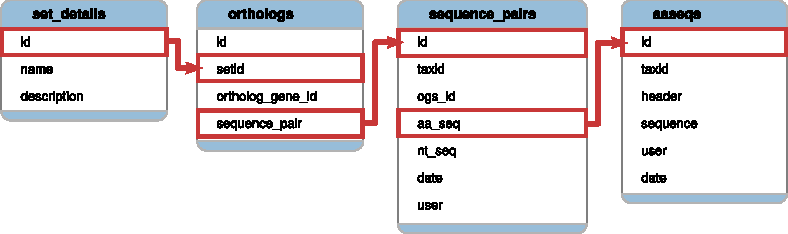
\includegraphics{img/db-orthoset.pdf}
	\caption[Database table connections for a given ortholog set]{
		\pname database structure for a given ortholog set. Each rounded rectangle
		represents a table with named columns. The red path delineates the
		\code{JOIN} query structure that returns all amino acid sequences (stored in
		the table ``aaseqs'') that belong to a given ortholog set. Ortholog set
		information is stored in the table ``set\_details''.
	}
	\label{fig:db-orthoset}
\end{figure}


\begin{figure}[ht]
	\centering
	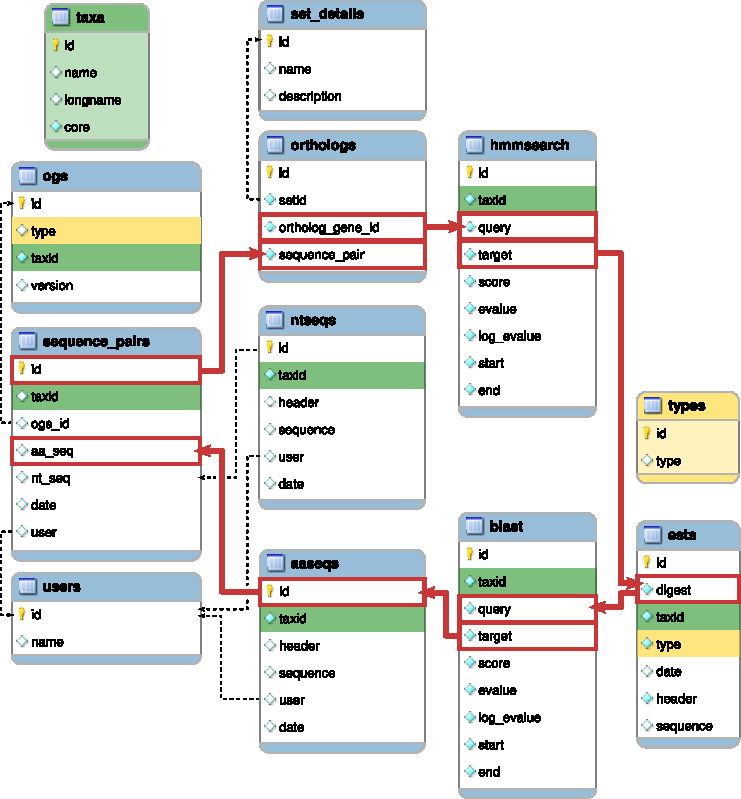
\includegraphics[width=\textwidth]{img/dbstructure.pdf}
	\caption[\pname database structure]{
		\pname database structure. Each rectangle represents a table with named
		columns. Note the circular path (red) that can be drawn across the tables and
		that is used in \code{JOIN} queries in order to construct a graph of
		orthologous relationships. Green table columns are referenced to the ``taxa''
		table, and yellow table columns are referenced to the ``types'' table. Dotted
		lines are secondary references.
	}
	\label{fig:dbstructure}
\end{figure}




	\section{Algorithm}
		\subsection{Analysis}
			The analysis algorithm is as follows:

\begin{enumerate}
	\item Get configuration, initialize global variables.
	\item Check the following:
	\begin{enumerate}
		\item Do the user settings make sense? If not, exit.
		\item Are the paths to the input file and the programs correct? If not,
			exit.
		\item Do the output directories exist? If not, create them.
		\item Does the database structure exist? If not, exit.
	\end{enumerate}
	\item Backup old results, if requested.
	\item Clear old results from file system and database, if requested.
	\item Create the HMMs, if they do not exist.
	\item Create the BLAST database of all core taxa, if it does not exist.
	\item Translate the input file in all six reading frames, if it is nucleic
		acid data.
	\item Load the translated sequences into the database, generating unique
		SHA256 digests on the way.
	\item Get all translated sequences of the target species from the database.
		Sequence identifiers are now SHA256 digests. Write the sequences into a
		temporary file.
	\item For each HMM, do the following:
	\begin{enumerate}
		\item Search the translated sequences in the temporary file with this HMM.
			Skip to the next HMM if no hits were obtained. Otherwise, read the tabular
			search report and store it in the database. 
		\item For each hit, do the following:
		\begin{enumerate}
			\item Get the hit sequence from the database and write the relevant
				subsequence to a Fasta file. This information has been gained from the
				hmmsearch report file.
			\item Search this sequence against the BLAST database. Skip to the next
				HMM if no hits were obtained. Otherwise, read the tabular search report
				and store it in the database. 
		\end{enumerate}
	\end{enumerate}
\end{enumerate}

Note that the analysis algorithm does not imply ortholog relationships. Only the
bidirectional searches are performed during this step. 

		\subsection{Reporting}
			\label{sec:algorithm-reporting}
The reporting algorithm is as follows:

\begin{enumerate}
	\item Get configuration, initialize global variables.
	\item Get a list of ortholog group IDs and their associated ortholog sequences
		from the database.
	\item Get all results in the form:
	\begin{lstlisting}
	hmmsearch_evalue => {
		ortholog_group_id => [
			reciprocal_hit,
			reciprocal_hit,
		],
		ortholog_gene_id => [
			reciprocal_hit,
			reciprocal_hit,
		],
		...
	}
	\end{lstlisting}
	\item Sort the e-values in ascending order.
	\item Starting with the lowest hmmsearch e-value, do the following:
	\begin{enumerate}
		\item For each ortholog group that has a hit with this e-value, do the following:
		\begin{enumerate}
			\item Check whether this ortholog group is present in the list that was
				generated in step 2. If not, skip to the next group (this ortholog group
				has already been assigned a transcript).
			\item Sort the reciprocal hits by BLAST e-value in ascending order.
			\item For each reciprocal hit, do the following:
			\begin{enumerate}
				\item If the reciprocal search hit a sequence that is in this ortholog
					group, and this transcript has not been assigned previously, then this
					is a valid match. Otherwise, skip to the next reciprocal hit unless
					the ``soft threshold'' has been reached (in that case, skip to the
					next ortholog group).
				\item Assign this transcript to this ortholog group if it does not
					overlap with an existing assignment. This transcript cannot be
					assigned again.
			\end{enumerate}
			\item If there is a gap between the transcripts (the end of one transcript
				lies more than 1 bp before the start of the next), fill the gap with
				'X' and concatenate the fragments.
		\end{enumerate}
	\end{enumerate}
\end{enumerate}


	\section{Implementation decisions}
		\subsubsection{Traversing the hit list by e-value}
		\subsubsection{Removing hits from the candidate list eliminates redundancy}

In order to avoid redundant assignment, \ie, a single transcript being assigned
to multiple ortholog groups or vice versa, candidate pairs that have been
verified are removed from the list of candidates. 

\begin{figure}[h]
	\centering
	\def\svgwidth{0.8\textwidth}
	\input{img/orthograph_graph.pdf_tex}
	\caption[Non-redundant assignment of ortholog relationships]{
		Non-redundant assignment of ortholog relationships. The ortholog groups (OG)
		are connected to the candidate hit transcripts by the e-value of the HMM
		search. Traversing the graph by ascending e-value and assigning the
		transcripts to the OG with the best hit results in transcript 3 being
		assigned to OG B, transcript 4 to OG C and transcript 2 to OG A. Transcript
		1 remains unassigned because the \tool{hmmsearch} e-value for OG A is higher than
		the e-value for transcript 2.
	}
	\label{fig:orthograph-graph}
\end{figure}



	\section{Performance tweaks}
		\subsection{One BLAST database comprising all core taxa proteomes}
			\pname uses a single BLAST database comprising all reference taxa proteomes.
Only one BLAST search is performed for each HMM hit.

		\subsection{RBDMS vs. flat files}
		\subsection{MySQL performance}
		\subsubsection{Individual tables per query species}
			During testing, it became obvious that not only the indexing strategy and the
query design, but also the database structure plays a major part in terms of
performance. Especially the tables ``ests'', ``hmmsearch'' and ``blast'' become
excessively large after a few analyses: assume a number of 500,000 transcript
sequences that are uploaded and an ortholog set of 4,000 OGs. If each of the
4,000 HMM searches obtains an average of 20 hits during the HMM search, and each
of the 20 BLAST searches obtain an average of 50 hits, this amounts to $4,000
\cdot 20 = 8 \cdot 10^4$ rows in the table ``hmmsearch'' and $4 \cdot 10^6$ rows in the
table ``blast''. The rows themselves do not contain much data (131 B
on average), but their sheer number brings InnoDB performance to its knees.
Insertion of new data does not become noticably slow, but the deletion of
unneeded records in the event of a repeated analysis that clears previous
results from the same query species from the database prior to the actual
analysis. The InnoDB cluster index physically orders the table based on the
primary key or the first unique key it can utilize. When one row is removed, the
entire table is reordered on disk for speed and defragmentation. With increasing
table size, this operation takes exponentially long \todo{data from hymenoptera:
transaction time}.

From what I have learned, the simplest and most performant solution to this
problem is to create individual tables for each query taxon. Dropping or
truncating (emptying) a table and recreating it is much faster than deleting a
large portion out of a huge table. 

	\section{SHA-256 checksums as sequence identifiers}
		Unique sequence IDs are necessary in order for \code{hmmsearch} not to create
confusion by treating whitespace in sequence headers as a description
separator. To avoid this, and to maintain a consistent naming scheme across
applications, \pname~uses a SHA-256 checksum to generate a unique ID for every
sequence. The checksum is generated using both the original header and the
sequence. Sequences are loaded into the database along with these checksums.
During the analysis, wherever a file is generated that includes sequence
identifiers, this checksum is used. This also eliminates the problem with
\code{fastatranslate} introducing whitespace that might confuse
\code{hmmsearch}.

It must be guaranteed that no two checksums, i.e., two sequence identifiers, are
ever the same. The SHA-256 hashing algorithm generates a checksum that is 160 bits,
or 40 hexadecimal characters in length. The probability $p$ of a hash collision
(i.e., two hashed elements returning the same checksum) in $n$ elements is

\begin{equation}
p \ge \frac{n (n-1)}{2} \times \frac{1}{2^b}
\label{eq:hashcollision}
\end{equation}

where $b$ is the number of bits generated by the hash function. There need to be
more than $1.7 \times 10^{15}$ objects for the SHA-256 hashes to exceed a collision
probability of $10^{-18}$. Since the hash space is expected to contain only a
number of objects in the range of $10^6$ to $10^{12}$, it is statistically safe
to assume that every checksum is unique. 



	\section{Benchmarks}

\chapter{Discussion and outlook}
	The results are of theoretical and practical nature and shed light on how a
pipeline for orthology prediction using HMMs and a RDBMS should be designed,
including challenges and pitfalls. 
The results also highlight the high potential of an extensive, metadata-enriched
ortholog cluster graph for phylogenetic and other analyses. 

During the development of \pname, I was faced with obstacles of both theoretical
and practical nature. I gained insights into the delicacies of modern Perl
development and high-performance MySQL database implementations.

	\section{Summary}
	\section{Comparisons with \hamstr}
	\section{Conclusion and outlook}

\phantomsection
\addcontentsline{toc}{chapter}{Bibliography}
% uncomment these two lines if using bibtex
\bibliographystyle{plainnat}
\bibliography{bib/diploma}
% uncomment this line if using biblatex
%\printbibliography
\clearpage

\phantomsection
\addcontentsline{toc}{chapter}{List of figures}
\listoffigures
\clearpage

\phantomsection
\addcontentsline{toc}{chapter}{List of tables}
\listoftables
\clearpage

\phantomsection
\appendix
\chapter{Appendix}
	\section{Listings}
		%\lstinputlisting[caption=Inserting random nucleotides at random intervals at a given probability, label=lst:randomframeshifts]{scripts/insertrandomframeshifts.pl}


\phantomsection
\chapter*{Acknowledgements}
	I thank Bernhard Misof for commiting this project to me, for helpful comments
and for maintaining such a great atmosphere in this working group.

Thanks to Oliver Niehuis for really good supervising and helpful discussions.
Your challenges made me outgrow my own boundaries.

I also thank Karen Meusemann for being a brilliant office-mate, for interesting
discussions, and for forming a great team. You made my diploma year.

Thanks to Alex Donath, Julia Schwarzer, Sandra Meid, Patrick Kück, Caro Greve,
Ralph Peters, Christoph Mayer, Jeanne Wilbrandt, Tanja Ziesmann, and Hannes
Jäkel for contributing to a good working group. Without all of you this year
wouldn't have been the same.

I also acknowledge Torsten Struck, who was the first to point out the redundant
assignment bug in \hamstr, and the helpful programming community at
\url{stackoverflow.com}, which helped me with tough questions concerning Perl
and MySQL, as well as Peter Grobe, whose concrete advice helped in designing the
database.

Thanks to Silvio Philipp as well as Alf and Monika Sibla for their friendship
and for taking my mind off everything else for a few hours each Wednesday. 

Many thanks to Hannah for making me smile every day, taking care of everything
and enduring my absent-mindedness the last few weeks. 

	\clearpage

\phantomsection
\addcontentsline{toc}{chapter}{Declaration of authorship}
\chapter*{Declaration of authorship}
	Ich versichere hiermit an Eides statt, dass die vorliegende Diplomarbeit
selbstständig verfasst und keine weiteren als die angegebenen Hilfsmittel
benutzt sowie die Stellen der Arbeit, die in anderen Werken dem Wortlaut oder
dem Sinn nach entnommen sind, durch Angaben der Quellen sichtbar gemacht
wurden.

\vspace{4em}

\parbox[t]{0.3\textwidth}{\dotfill}

Bonn, \today

\vspace{8em}

\author

\end{document}
